\documentclass{article}
\usepackage{tikz}
\usetikzlibrary{shapes, positioning}
\usepackage{amssymb} % Needed for \mathbb

\begin{document}


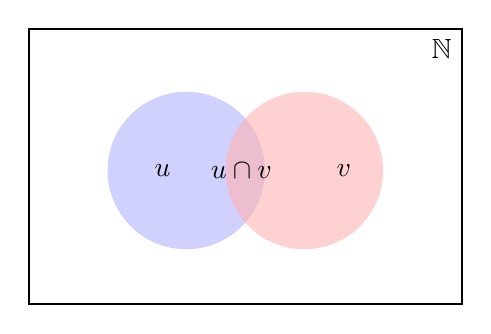
\begin{tikzpicture}
  % Rectangle representing N
  \draw[thick] (-1.5,-1.5) rectangle (4,2) node[anchor=north east] {$\mathbb{N}$};

  % Set u
  \fill[blue!30, opacity=0.6] (0.5,0.2) circle (1.0cm);
  \node at (0.2,0.2) {$u$};

  % Set v with small intersection
  \fill[red!30, opacity=0.6] (2.0,0.2) circle (1.0cm);
  \node at (2.5,0.2) {$v$};

  % Optional: label the intersection
  \node at (1.2,0.2) {$u \cap v$};
\end{tikzpicture}

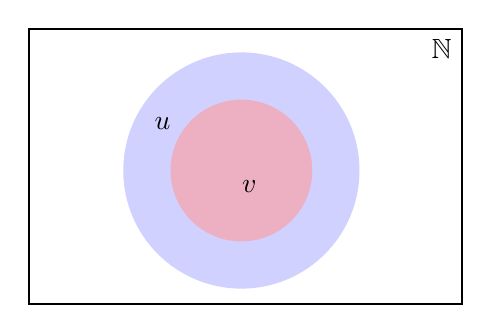
\begin{tikzpicture}
  % Rectangle for N
  \draw[thick] (-1.5,-1.5) rectangle (4,2) node[anchor=north east] {$\mathbb{N}$};

  % Set u (outer)
  \fill[blue!30, opacity=0.6] (1.2, 0.2) circle (1.5cm);
  \node at (0.2,0.8) {$u$};

  % Set v (nested inside)
  \fill[red!40, opacity=0.6] (1.2,0.2) circle (0.9cm);
  \node at (1.3,0) {$v$};
\end{tikzpicture}

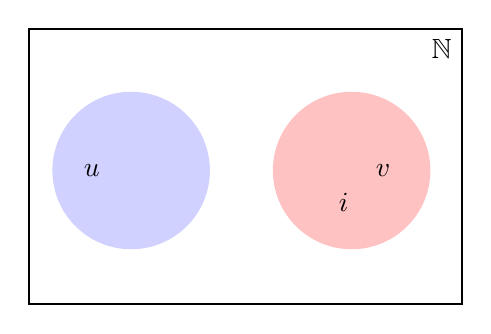
\begin{tikzpicture}
  % Rectangle for N
  \draw[thick] (-1.5,-1.5) rectangle (4,2) node[anchor=north east] {$\mathbb{N}$};

  % Set u (left)
  \fill[blue!30, opacity=0.6] (-0.2,0.2) circle (1.0cm);
  \node at (-0.7,0.2) {$u$};

  % Set v (right), disjoint from u
  \fill[red!40, opacity=0.6] (2.6,0.2) circle (1.0cm);
  \node at (3.0,0.2) {$v$};

  % Index i inside v
  \node at (2.5,-0.2) {$i$};
\end{tikzpicture}



\end{document}

